\documentclass{classrep}
\usepackage[utf8]{inputenc}
\usepackage{color}
\usepackage{enumitem}
\usepackage{graphicx}
\usepackage{amsmath}
\usepackage{float}
\usepackage{hyperref}
\usepackage{environ}
\usepackage{comment}
\usepackage{amsmath}
\usepackage{amssymb}
\usepackage{amsthm}
\usepackage{longtable}
\usepackage{lscape}
\usepackage{icomma}
{\theoremstyle{definition}
  \newtheorem{definition}{Definicja}
}

\studycycle{Informatyka, studia dzienne, I st.}
\coursesemester{VI}

\coursename{Komputerowe systemy rozpoznawania}
\courseyear{2019/2020}

\courseteacher{dr hab. inż. Adam Niewiadomski prof. uczelni}
\coursegroup{pon., 12:15}

\author{
\studentinfo{Mateusz Walczak}{216911} \and
\studentinfo{Konrad Kajszczak}{216790}
}

\title{Zadanie 2: Lingwistyczne podsumowania baz danych}
\svnurl{https://github.com/Walducha1908/KSR2}

\begin{document}
\maketitle

\section{Cel}
Celem zadania było zaprojektowanie aplikacji desktopowej, służącej do generowania podsumowań lingwistycznych oraz obliczania ich miar jakości dla wybranej bazy danych. Dodatkowo, aplikacja powinna posiadać graficzny interfejs użytkownika, który umożliwi intuicyjne korzystanie z programu.


\section{Wprowadzenie}
Rozważania we wprowadzeniu rozpoczniemy od \emph{zbioru rozmytego}, czyli najbardziej podstawowego pojęcia, bez którego analiza działania ingwistycznych podsumowań baz danych nie byłaby mozliwa. Przytoczmy zatem definicję \emph{zbioru rozmytego}:

\begin{definition}
Niech \(\mathcal{X}\) będzie zbiorem, którego elementy interesują
nas w sposób bezpośredni, czyli jest zbiorem klasycznym znanym z teorii mnogości (dany element przynależy do zbioru lub nie przynależy).
Wówczas \emph{zbiorem rozmytym opisanym w przestrzeni rozważań \(\mathcal{X}\)}
nazywamy każdy zbiór \(A\) postaci:
\[A = \bigcup_{x \in \mathcal{X}} \{(x,\, \mu_A(x))\},\]
gdzie \(\mu_A(x) : \mathcal{X} \to [0,\,1]\) nazywamy \emph{funkcją
przynależności do zbioru rozmytego \(A\)}.
\end{definition}

W związku z faktem, iż pojęcie \emph{funkcji przynależności} wystąpiło w powyższej definicji, w następnym podrozdziale zajmiemy się opisem tego rodzaju funkcji, wykorzystywanych przez nas.



\subsection{Funkcje przynależności}

Funkcja przynależności określa w jakim stopniu dany element przynależy do zbioru. W zbiorach rozmytych zakres wartości jakie może ona przyjmować jest rozszerzony do przedziału [0,1]. \newline

W naszym programie, posłużyliśmy się dwoma rodzajami funkcji przynależności:

\begin{itemize}[label=$\bullet$\scshape\bfseries]
\item funkcją trójkątną opisaną wzorem:
\begin{equation}
{f}_{troj}(x)= \left\{ \begin{array}{ll}
\frac{x-a}{b-a} 	& \textrm{jeśli $a \leq x < b$} \\
1 			& \textrm{jeśli $ x = b $} \\
\frac{c-x}{c-b} 	& \textrm{jeśli $b < x \leq v$} \\
0 			& \textrm{w przeciwnym wypadku.} \\
\end{array} \right.
\end{equation}


\item oraz funkcją trapezoidalną opisaną wzorem:

\begin{equation}
{f}_{trap}(x)= \left\{ \begin{array}{ll}
\frac{x-a}{b-a} 	& \textrm{jeśli $a \leq x < b$} \\
1 			& \textrm{jeśli $b \leq x \leq c$} \\
\frac{d-x}{d-c} 	& \textrm{jeśli $c < x \leq d$} \\
0 			& \textrm{w przeciwnym wypadku.} \\
\end{array} \right.
\end{equation}


\end{itemize}

gdzie $a$, $b$, $c$ oraz $d$ są parametrami funkcji przynależności - wierzchołkami trójkąta lub trapezu na wykresie.




\subsection{Miary jakości dla podumowań lingwistycznych}

Aby określić jakość naszych podsumowaniań zaimplementowaliśmy 11 miar jakości od $T_1$ do $T_{11}$ \cite{ksiazka}.

\subsubsection{\(T_1\) -- stopień prawdziwości}

Stopień prawdziwości jest najbardziej naturalną miarą jakości podsumowania. Określa ona sumę przynależności wszystkich rozważanych krotek do sumaryzatora \(S_j\):
\[r = \sum_{i=1}^{m} \mu_{\mathrm{ce}(S_j)}(d_i) ~\mbox{,}\]
gdzie \(\mathrm{ce}(S_j)\) jest rozszerzeniem cylindrycznym
sumaryzatora \(S_j\), \(m\) liczba wszystkich krotek, a \(d_i\).
Dla kwantyfikatorów relatywnych stopnień
prawdziwości możemy zapisać jako
$$T_1 = \mu_Q(\frac{r}{m}),$$
zaś dla kwantyfikatorów absolutnych jako
$$T_1 = \mu_Q(r),$$
gdzie \(r\) jest kardynalnością. 

\subsubsection{\(T_2\) -- stopień nieprecyzyjności}
Dla podsumowania z \(n\) sumaryzatorami \(S_1 \ldots S_n\) możemy określić stopień nieprecyzyjności,
definiowany następującym wzorem:
\[T_2 = 1 - \left(\prod_{j=1}^{n} \mathrm{in}(S_j)\right)^{1/n} ~\mbox{.}\]
Wyrażenie \(\left(\prod_{j=1}^{n} \mathrm{in}(S_j)\right)^{1/n}\) to określa średnią geometryczna ze stopni rozmycia wykorzystanych sumaryzatorów, czyli w jakim stopniu precyzyjny jest sumaryzator. Im mniejszy nośnik zbioru rozmytego, tym wyższa jest jego precyzja.
   

\subsubsection{\(T_3\) -- stopień pokrycia}
Stopień pokrycia \(T_3\) jest zdefiniowany dla podsumowań z kwalifikatorami. Stopień pokrycia $T_3$ 
Dla każdego \(i=1\ldots m\) (związanego z krotką \(d_i\) z bazy
danych) możemy zdefiniować (z kwalifikatorem):
\[
\begin{array}{l}
t_i = \begin{cases}
1 & \mbox{gdy } \mu_{\mathrm{ce}(S_j)}(d_i) > 0 ~ \wedge ~ \mu_{W}(d_i) > 0 \\
0 & \mbox{w przeciwnym wypadku.}
\end{cases} \\
h_i = \begin{cases}
1 & \mbox{gdy } \mu_{W}(d_i) > 0 \\
0 & \mbox{w przeciwnym wypadku.}
\end{cases}
\end{array}\]

Bez kwalifikatora:

\[
\begin{array}{l}
t_i = \begin{cases}
1 & \mbox{gdy } \mu_{\mathrm{ce}(S_j)}(d_i) > 0  \\
0 & \mbox{w przeciwnym wypadku.}
\end{cases} \\
\end{array}\]
\[h_1 = 1\]

Przy powyższych oznaczeniach:
\[T_3 = \frac{\sum_{i=1}^{m} t_i}{\sum_{i=1}^{m} h_i} ~\mbox{.}\]

Reprezentuje stopień w jakim nośnik sumaryzatora pokrywa się z nośnikiem kwalifikatora.


\subsubsection{\(T_4\) -- stopień trafności}
Dla podsumowania z \(n\) sumaryzatorami \(S_1 \ldots S_n\)
oraz \(m\) krotkami w bazie danych możemy wprowadzić oznaczenia:
\[g_{ij} = \begin{cases}
1 & \mbox{gdy } \mu_{\mathrm{ce}(S_j)}(d_i) > 0 \\
0 & \mbox{w przeciwnym wypadku.}
\end{cases}\]
oraz
\[r_j = \frac{\sum_{i=1}^{m} g_{ij}}{m} ~\mbox{.}\]
Wówczas możemy zapisać:
\[T_4 = \left| \prod_{j=1}^{n} r_j - T_3\right| ~\mbox{.}\]

 Określa jak wiele krotek przynależy do sumaryzatora, czyli czy dane podsumowanie jest właściwe dla zestawu danych.

\subsubsection{\(T_5\) -- długość podsumowania}
Dla podsumowania z \(n\) sumaryzatorami \(S_1 \ldots S_n\)
miarę długości podsumowania definiujemy jako:
\[T_5 =  2 \left(\frac{1}{2}\right)^{|s|} ~\mbox{.}\]

Gdzie \(|s|\) jest ilością zbiorów rozmytych,z  których skomponowany jest sumaryzator. Określa jakość podsumowania na podstawie złożoności sumaryzatora, czyli im więcej składowych sumaryzatora złożonego, tym niższa wartość tej miary.

\subsubsection{\(T_6\) -- stopień nieprecyzyjności kwantyfikatora}
\(T_6\), czyli stopień nieprecyzyjności kwantyfikatora możemy zdefiniować jako:

\[T_6 = 1-\mathrm{in}(Q) ~\mbox{.}\]

Reprezentuje w jakim stopniu precyzyjny jest kwantyfikator. Im mniejszy nośnik zbioru rozmytego tym wyższa jest jego precyzja.

\subsubsection{\(T_7\) -- stopień liczności kwantyfikatora}
W przeciwieństwie do \(T_6\), zamiast zliczać elementy z nośnika \(Q\),
policzymy moc zbioru rozmytego:
\[T_7 = 1-\frac{|Q|}{|\mathcal{X}_Q|} ~\mbox{.}\]

Opisuje stopień precyzji kwantyfikatora, im mniejsza kardynalność kwantyfikatora tym jest on bardziej precyzyjny.

\subsubsection{\(T_8\) -- stopień liczności sumaryzatora}
W przypadku zastosowania sumaryzatora złożonego, podobnie jak przy poprzednich miarach, stosujemy średnią geometryczną.
Dla podsumowania z \(n\) sumaryzatorami \(S_1 \ldots S_n\):

\[T_8 = 1- \left(\prod_{j=1}^{n} \frac{|S_j|}{|\mathcal{X}_j|}\right)^{\frac{1}{n}} ~\mbox{.}\]

Opisuje stopień precyzji sumaryzatora, im mniejsza kardynalność kwantyfikatora tym jest on bardziej precyzyjny.

\subsubsection{\(T_9\) -- stopień nieprecyzyjności kwalifikatora}
Stopień precyzji kwalifikatora \(T_9\) jest oparty na drugiej formie podsumowań tzn.: Q obiektów będących/mających W jest/ma S, gdzie W jest reprezentowane przez zbiór rozmyty i jest kwalifikatorem. Definicja tej miary jest następująca:
\[T_9 = 1-\mathrm{in}(W) ~\mbox{.}\]

Określa w jakim stopniu precyzyjny jest kwalifikator. Im szerszy nośnik zbioru rozmytego tym niższa jest jego precyzja, gdyż bierze pod uwagę większy zakres wartości. 


\subsubsection{\(T_{10}\) -- stopień liczności kwalifikatora}
Stopień kardynalności kwalifikatora \(T_{10}\) definiujemy jako:
\[T_{10} = 1-\frac{|W|}{|\mathcal{X}_g|} ~\mbox{.}\]\\

Opisuje stopień precyzji kwalifikatora, im większa jest kardynalność kwalifikator tym jest on mniej precyzyjny.

\subsubsection{\(T_{11}\) -- długość kwalifikatora}
Długość kwalifikatora \(T_{11}\) definiujemy następująco:
\[T_{11} = 2\left(\frac{1}{2}\right)^{|W|} ~\mbox{.}\]

Wyznacza jakość podsumowania na podstawie złożoności kwalifikatora, Im bardziej złożony kwalifikator tym jakość podsumowania gorsza.

\clearpage



\section{Opis implementacji}

Program został napisany w języku Java z wykorzystaniem narzędzia Maven \cite{Maven}, służącego do automatyzacji budowy oprogramowania. Graficzny interfejs użytkownika został zbudowany w oparciu o bibliotekę JavaFX \cite{FX}.\newline

W opisie implementacji skoncentrujemy się na jej najważniejszej części, czyli logice aplikacji.\newline 

W celu zbudowania struktury klas reprezentujących typy, parametry i własności zbiorów rozmytych oraz operacji na nich, zaimplementowaliśmy własną bibliotekę w formie pakietu w naszej aplikacji o nazwie \textit{FuzzyLib}.\newline

Pakiet \textit{FuzzyLib} został podzielony na następujące podpakiety:
\begin{itemize}[label=$\bullet$\scshape\bfseries]
\item  \textit{Membership},
\item  \textit{Logic},
\item  \textit{Containers},
\item  \textit{Summaries}.
\end{itemize}

W tym rozdziale omówione zostaną wszystkie wyżej wymienione podpakiety. Przedstawimy diagramy UML każdego z podpakietów a także omówimy zastosowanie poszczególnych klas.

\subsection{Podpakiet Membership}
Podpakiet \textit{Membership} zawiera implementacje funkcji przynależności. Każda klasa tego podpakietu implementuje interfejs  \textit{MembershipFunction}.

\begin{figure}[H]
	\centering
	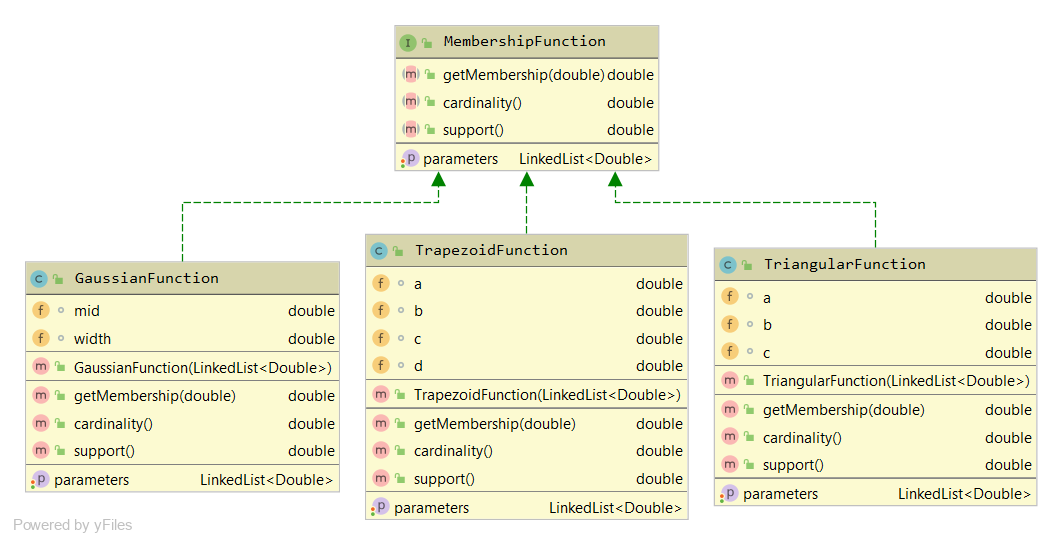
\includegraphics[width=1\textwidth]{{Pictures/Diagrams/Membership.png}}
	\caption{Diagram UML dla podpakietu \textit{Membership}}
\end{figure}

Klasy podpakietu \textit{Membership} są następujące:
\begin{itemize}[label=$\bullet$\scshape\bfseries]
\item \textit{MembershipFunction} - interfejs implementowany przez wszystkie klasy należące do tego podpakietu,
\item \textit{TriangularFunction} - klasa implementująca trójkątną funkcję przynależności,
\item \textit{DescreteFunction} - klasa implementująca dyskretną funkcję przynależności,
\item \textit{ConstantFunction} - klasa implementująca stałą funkcję przynależności,
\item \textit{TrapezoidFunction} - klasa implementująca trapezoidalną funkcję przynależności.
\end{itemize}



\subsection{Podpakiet Logic}
Podpakiet \textit{Logic} odpowiada za implementacje zmiennych lingwistycznych, operacji sumy i iloczynu zbiorów rozmytych a także miar jakości podsumowań lingwistycznych.

\begin{figure}[H]
	\centering
	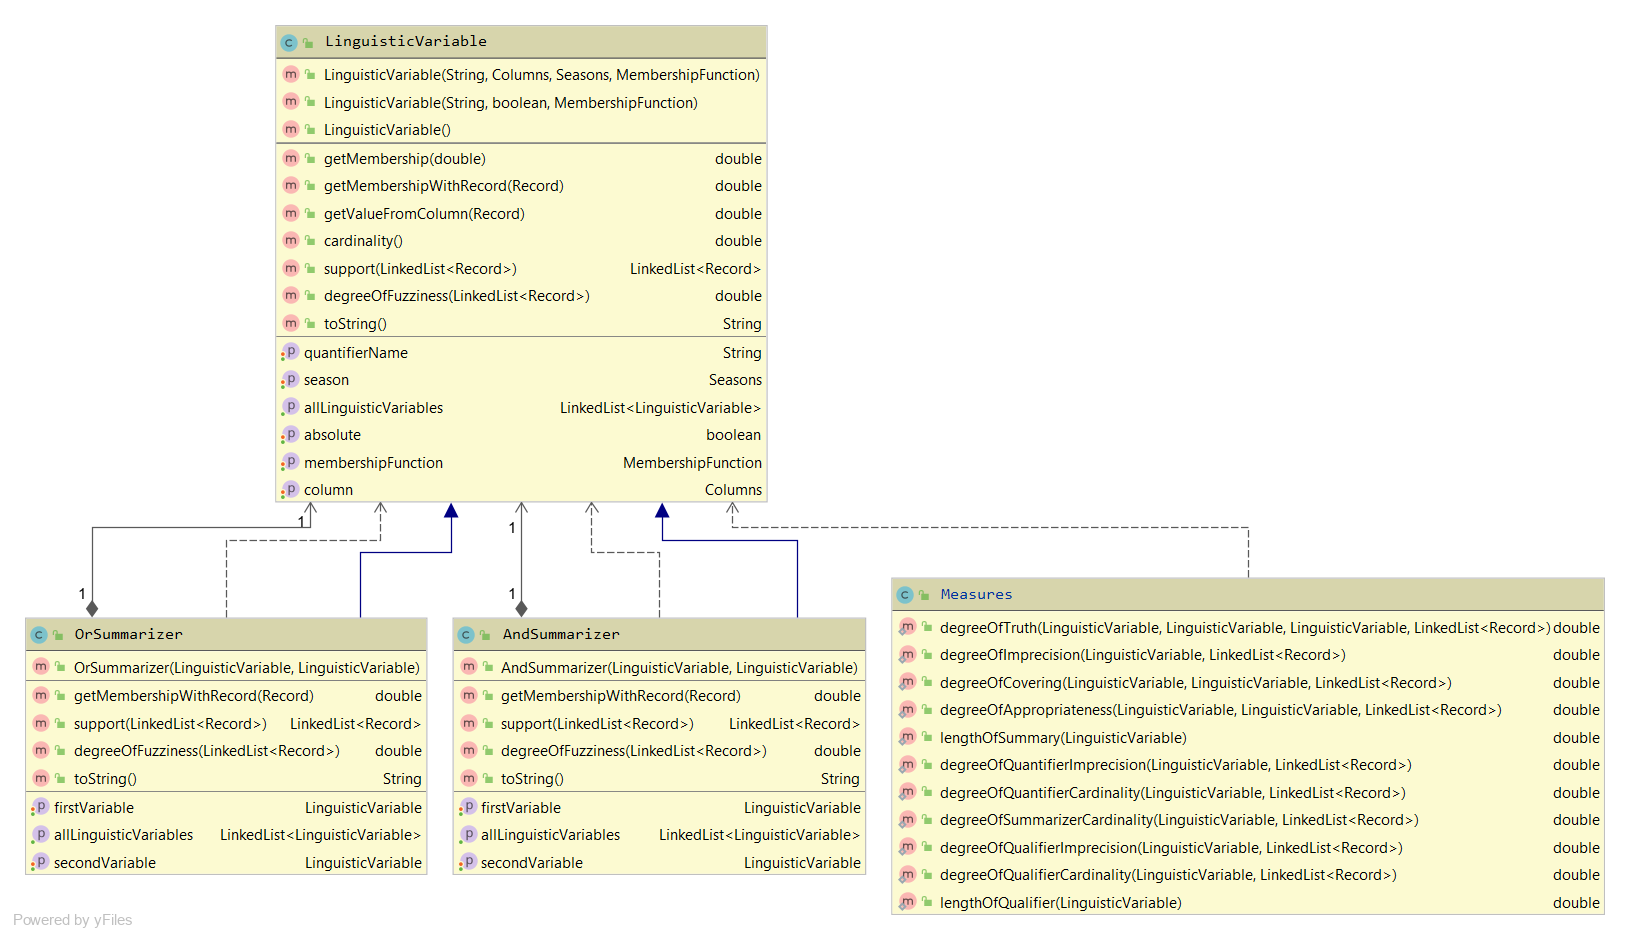
\includegraphics[width=1\textwidth]{{Pictures/Diagrams/Logic.png}}
	\caption{Diagram UML dla podpakietu \textit{Logic}}
\end{figure}

Klasy podpakietu \textit{Logic} są następujące:
\begin{itemize}[label=$\bullet$\scshape\bfseries]
\item \textit{LinguisticVariable} - klasa implementująca zmienną lingwistyczną,
\item \textit{AndSummarizer} - klasa implementująca operacje iloczynu, dziedziczy z klasy \textit{LinguisticVariable},
\item \textit{OrSummarizer} -  klasa implementująca operacje sumy, dziedziczy z klasy \textit{LinguisticVariable},
\item \textit{Measures} - klasa implementująca miary jakości podsumowań lingwistycznych.
\end{itemize}



\subsection{Podpakiet Containers}
Podpakiet \textit{Containers} zawiera klasy kontenerowe, tworzące i przetrzymujące zmienne lingwistyczne i kwantyfikatory.

\begin{figure}[H]
	\centering
	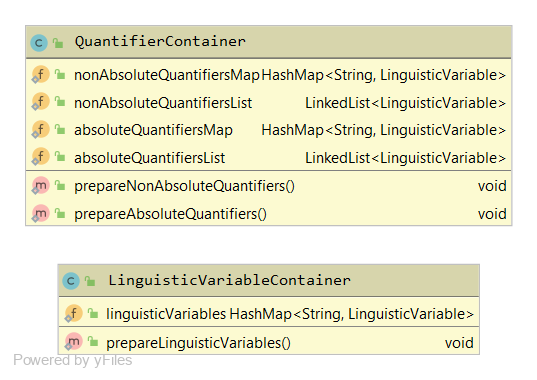
\includegraphics[width=0.65\textwidth]{{Pictures/Diagrams/Containers.png}}
	\caption{Diagram UML dla podpakietu \textit{Containers}}
\end{figure}

Klasy podpakietu \textit{Containers} są następujące:
\begin{itemize}[label=$\bullet$\scshape\bfseries]
\item \textit{LinguisticVariableContainer} - klasa kontenerowa dla zmiennych lingwistycznych,
\item \textit{QuantifierContainer} - klasa kontenerowa dla kwantyfikatorów.
\end{itemize}



\subsection{Podpakiet Summaries}
Podpakiet \textit{Summaries} zawiera dwie klasy odpowiadające za budowę zdań podsumowania lingwistycznego w języku ludzkim (angielskim) oraz obliczenie wszystkich miar jakości dla danego podsumowania lingwistycznego - wywołanie statycznych metod klasy \textit{Measures} podpakietu \textit{Logic}.

\begin{figure}[H]
	\centering
	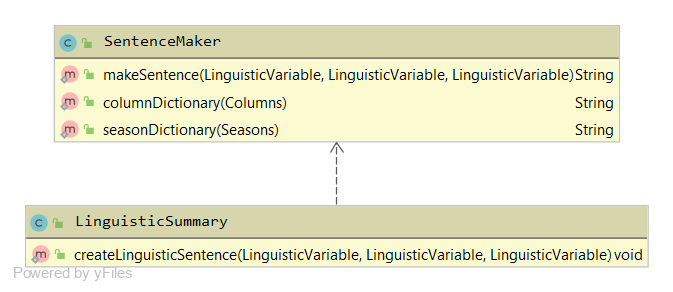
\includegraphics[width=0.85\textwidth]{{Pictures/Diagrams/Summaries.png}}
	\caption{Diagram UML dla podpakietu \textit{Summaries}}
\end{figure}

Klasy podpakietu \textit{Summaries} są następujące:
\begin{itemize}[label=$\bullet$\scshape\bfseries]
\item \textit{LinguisticSummary} - klasa odpowiadająca za obliczenie wszystkich miar jakości dla danego podsumowania,
\item \textit{SentenceMaker} - klasa odpowiadająca za budowanie zdań w języku ludzkim.
\end{itemize}

\clearpage




\section{Materiały i metody}
Wybrana przez nas baza danych zawiera historyczne pomiary pogodowe z Holandii \cite{baza}. Dane zostały zgromadzone przez KNMI (\textit{Dutch weather institute} - Holenderski instytut pogodowy) na przestrzeni lat 1901-2018 i pochodziły z 50 różnych stacji pogowych znajdujących się na terenie całego kraju.\newline

Ze względu na fakt, iż oryginalna baza danych składa się z 804099 krotek, postanowiliśmy wybrać tylko niewielką część z dostępnych danych. Zdecydowaliśmy się na najnowsze dane pomiarowe - z lat 2016-2018. W ten sposób ograniczyliśmy liczbę wykorzystywanych krotek do 17000.\newline

\subsection{Wybór kolumn}
W celu analizy bazy danych i tworzenia jej lingwistycznych podsumowań wybraliśmy 10 kolumn z danymi liczbowymi.

\begin{figure}[H]
	\centering
	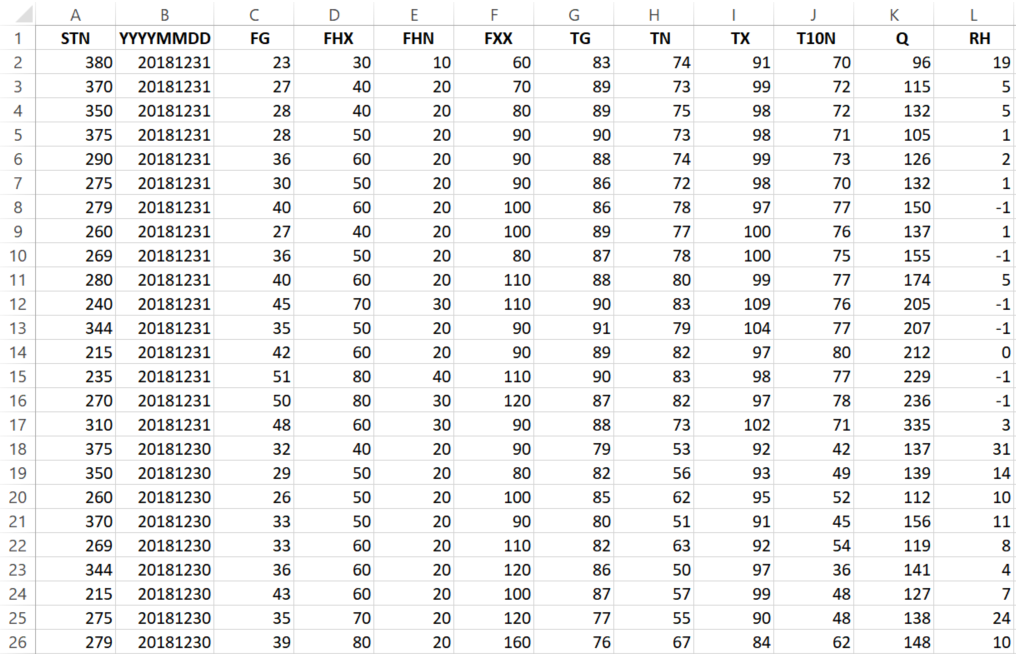
\includegraphics[width=\textwidth]{Pictures/baza.png}
	\caption{Fragment widoku bazy w formacie $xlsx$}
\end{figure}

Wybrane kolumny są następujące:
\begin{itemize}[label=$\bullet$\scshape\bfseries]
\item FG - średnia prędkość wiatru przez cały dzień [$0.1 \frac{m}{s}$].
\item FHX - najwyższa średnia prędkość wiatru w ciągu jednej godziny [$0.1 \frac{m}{s}$].
\item FHN - najniższa średnia prędkość wiatru w ciągu jednej godziny [$0.1 \frac{m}{s}$].
\item FXX - najszybszy podmuch wiatru w ciągu całego dnia [$0.1 \frac{m}{s}$].
\item TG - średnia dzienna temperatura [$0.1^{\circ} C$].
\item TN - minimalna dzienna temperatura [$0.1^{\circ} C$].
\item TX - maksymalna dzienna temperatura [$0.1^{\circ} C$].
\item T10N - minimalna dzienna temperatura na wysokości 10 cm od poziomu gruntu [$0.1^{\circ} C$].
\item Q - nasłonecznienie, energia słoneczna przypadająca na powierzchnię [$\frac{J}{cm^2}$].
\item RH - suma opadów atmosferycznych w ciągu całego dnia [$0.1 mm$].\newline
\end{itemize}

Oprócz wyżej opisanych danych liczbowych, w naszej bazie znajdują się także dwie dodatkowe kolumny, służące do identyfikacji pomiaru:
\begin{itemize}[label=$\bullet$\scshape\bfseries]
\item STN - numer stacji badawczej wykonującej pomiar.
\item YYYYMMDD - data pomiaru w formacie opisanym przez nazwę kolumny.
\end{itemize}




\subsection{Zmienne lingwistyczne}
W tym rozdziale przedstawimy wzory i wykresy opisujące zaproponowane przez nas zmiennie lingwistyczne. We wszystkich przypadkach, wykorzystywanymi przez nas funkcjami przynależności są funkcje trapezoidalne.  \footnote{Wartości prezentowane w tabelach są tylko propozycjami. Autorzy sprawozdania zastrzegają sobie możliwość do ich późniejszej modyfikacji}.\newline

Aby nie duplikować treści wzorów, niepotrzebnie zwiększając w ten sposób objętość sprawozdania, zdecydowano się na zamieszczenie tabel z parametrami etykiet zmiennych lingwistycznych, odnoszącymi się do wzorów z poprzedniego podrozdziału.

\clearpage



\subsubsection{Kolumna FG}
Wykres opisujący zmienną lingwistyczną dla kolumny zawierającej wartości średniej prędkości wiatru przez cały dzień (FG), zamieszczono poniżej.
\begin{figure}[H]
	\centering
	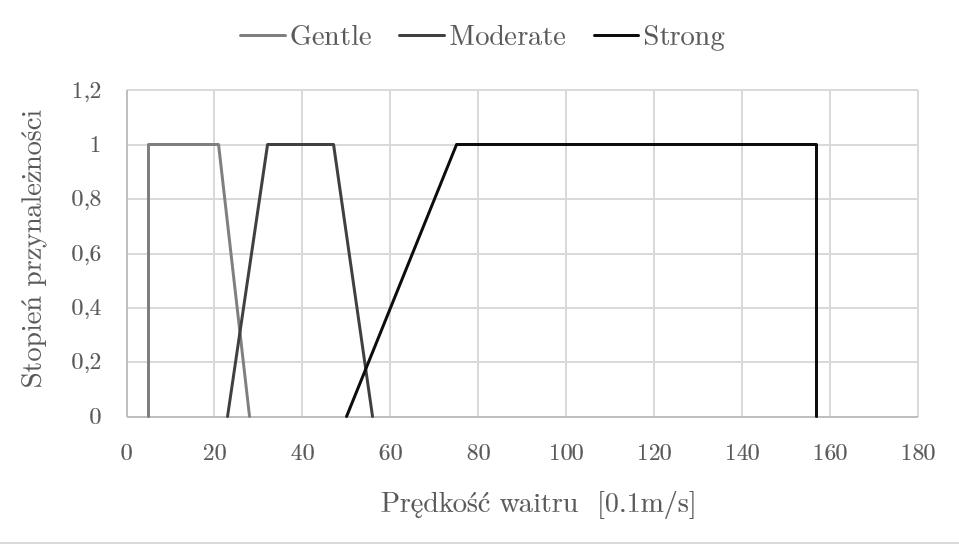
\includegraphics[width=0.99\textwidth]{Pictures/TermsCharts/FG.png}
	\caption{Wykres opisujący zmienną lingwistyczną dla kolumny FG.}
\end{figure}

\begin{table}[H]
	\centering
	\begin{tabular}{c c c c c} 
		\hline
		\textbf{Etykieta} & \textbf{a} & \textbf{b} & \textbf{c} & \textbf{d}\\ [0.5ex] 
		\hline
		\hline 
Gentle	 & 5 & 5 & 21 & 28 \\
Moderate & 23 & 32 & 47 & 56 \\
Strong	 & 50 & 75 & 157 & 157 \\
		\hline
	\end{tabular}
	\caption{Przyporządkowane parametry funkcji trapezoidalnej dla kolumny FG.}
\end{table}

\clearpage



\subsubsection{Kolumna FHX}
Wykres opisujący zmienną lingwistyczną dla kolumny zawierającej najwyższą średnią prędkości wiatru w przeciągu jednej godziny (FHX), zamieszczono poniżej.
\begin{figure}[H]
	\centering
	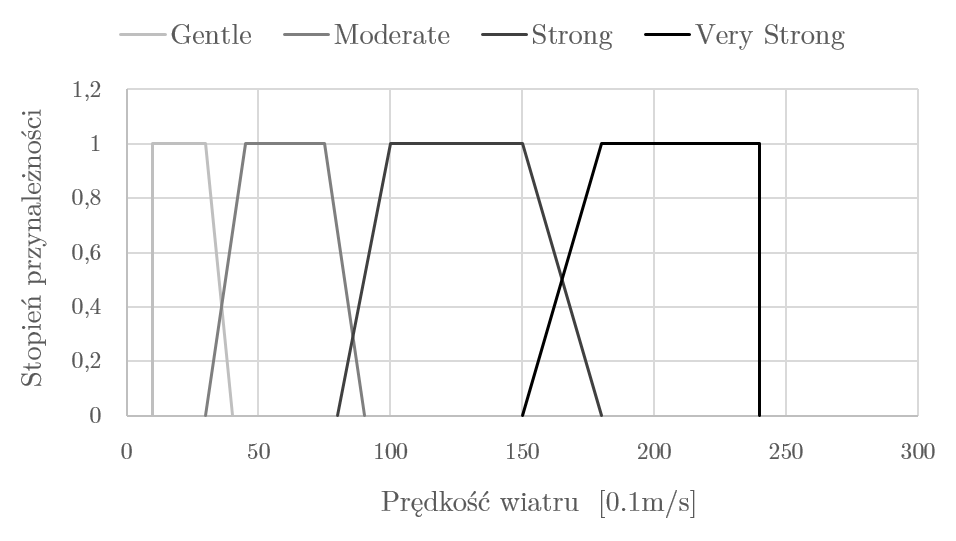
\includegraphics[width=0.99\textwidth]{Pictures/TermsCharts/FHX.png}
	\caption{Wykres opisujący zmienną lingwistyczną dla kolumny FHX.}
\end{figure}

\begin{table}[H]
	\centering
	\begin{tabular}{c c c c c} 
		\hline
		\textbf{Etykieta} & \textbf{a} & \textbf{b} & \textbf{c} & \textbf{d}\\ [0.5ex] 
		\hline
		\hline 
Gentle	 & 10 & 10 & 30 & 40 \\
Moderate & 30 & 45 & 75 & 90 \\
Strong	 & 80 & 100 & 150 & 180 \\
Very strong & 150 & 180 & 240 & 240 \\
		\hline
	\end{tabular}
	\caption{Przyporządkowane parametry funkcji trapezoidalnej dla kolumny FHX.}
\end{table}

\clearpage

\subsubsection{Kolumna FHN}
Wykres opisujący zmienną lingwistyczną dla kolumny zawierającej najniższą średnią prędkości wiatru w przeciągu jednej godziny (FHN), zamieszczono poniżej.
\begin{figure}[H]
	\centering
	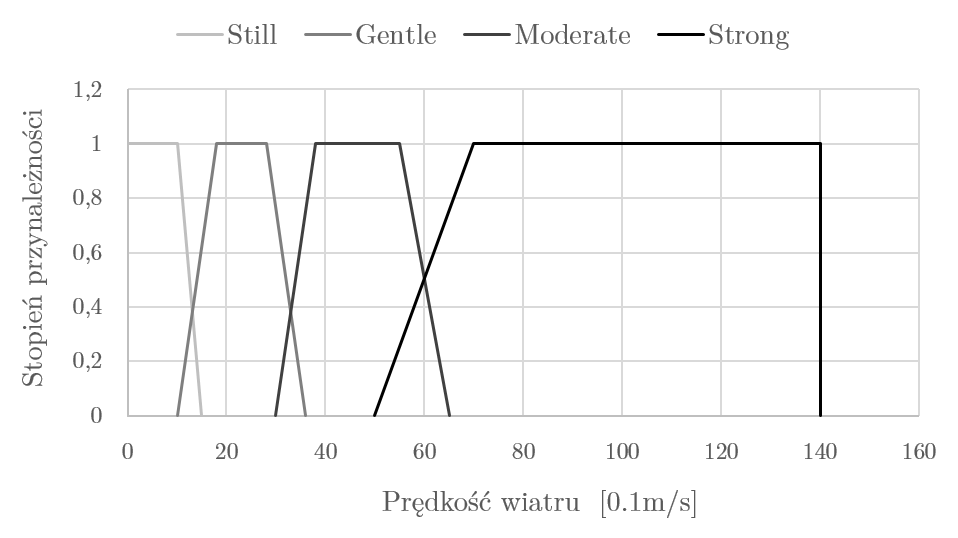
\includegraphics[width=0.99\textwidth]{Pictures/TermsCharts/FHN.png}
	\caption{Wykres opisujący zmienną lingwistyczną dla kolumny FHN.}
\end{figure}

\begin{table}[H]
	\centering
	\begin{tabular}{c c c c c} 
		\hline
		\textbf{Etykieta} & \textbf{a} & \textbf{b} & \textbf{c} & \textbf{d}\\ [0.5ex] 
		\hline
		\hline 
Gentle	 & 0 & 0 & 10 & 15 \\
Moderate & 10 & 18 & 28 & 36 \\
Strong	 & 30 & 38 & 55 & 65 \\
Very strong & 50 & 70 & 140 & 140 \\
		\hline
	\end{tabular}
	\caption{Przyporządkowane parametry funkcji trapezoidalnej dla kolumny FHN.}
\end{table}

\clearpage

\subsubsection{Kolumna FXX}
Wykres opisujący zmienną lingwistyczną dla kolumny zawierającej najsilniejszy powiew wiatru (FXX), zamieszczono poniżej.
\begin{figure}[H]
	\centering
	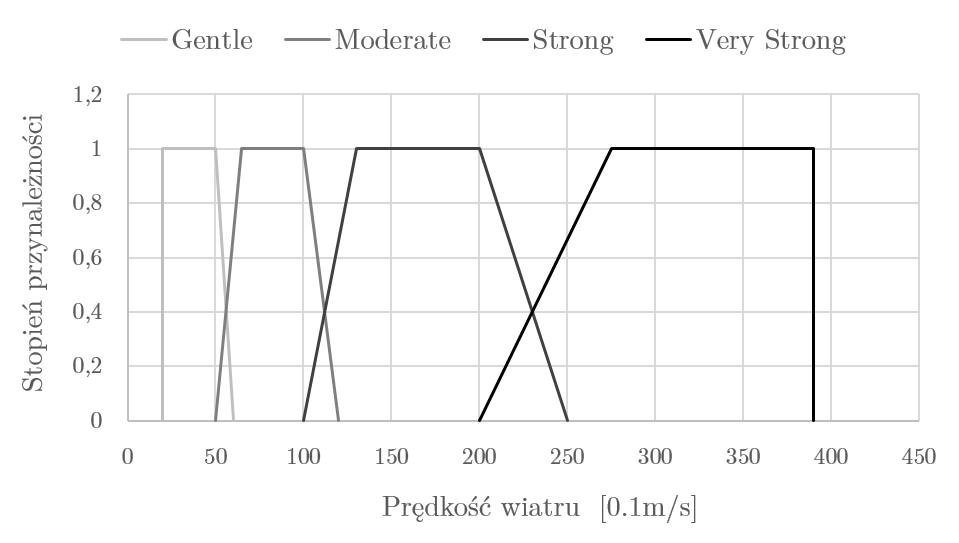
\includegraphics[width=0.99\textwidth]{Pictures/TermsCharts/FXX.png}
	\caption{Wykres opisujący zmienną lingwistyczną dla kolumny FXX.}
\end{figure}

\begin{table}[H]
	\centering
	\begin{tabular}{c c c c c} 
		\hline
		\textbf{Etykieta} & \textbf{a} & \textbf{b} & \textbf{c} & \textbf{d}\\ [0.5ex] 
		\hline
		\hline 
Gentle	 & 20 & 20 & 50 & 60 \\
Moderate & 50 & 65 & 100 & 120 \\
Strong	 & 100 & 130 & 200 & 250 \\
Very strong & 200 & 275 & 390 & 390 \\
		\hline
	\end{tabular}
	\caption{Przyporządkowane parametry funkcji trapezoidalnej dla kolumny FXX.}
\end{table}

\clearpage



\subsubsection{Kolumna TG}
W przypadku średniej dziennej temperatury (TG) oraz innych kolumn związacnyh z temperaturą (TN, TX oraz T10N), zdecydowaliśmy się podzielić nasze rozważania ze względu na pory roku. Dlatego też przyjęliśmy trzy różne warianty zmiennej lingiwstycznej dla kolumny TG:

\begin{itemize}[label=$\bullet$\scshape\bfseries]
\item TGW - dla pomiarów uzyskanych podczas astronomicznej zimy (litera $W$ od $Winter$),
\item TGSA - dla pomiarów uzyskanych podczas astronomicznej wiosny lub jesieni ($S$ od $Spring$, $A$ od $Autumn$),
\item TGS - dla pomiarów uzyskanych podczas astronomicznego lata (litera $S$ od $Summer$).\newline\newline
\end{itemize}

Rozpocznijmy od zmiennej lingwistycznej TGW.
\begin{figure}[H]
	\centering
	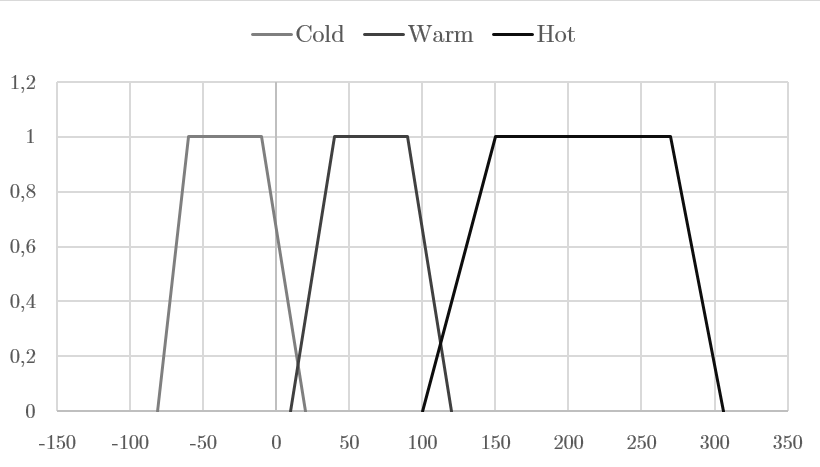
\includegraphics[width=0.99\textwidth]{Pictures/TermsCharts/TG_Z.png}
	\caption{Wykres opisujący zmienną lingwistyczną dla kolumny TG dla pomiarów wykonanych astronomiczną zimą.}
\end{figure}

\begin{table}[H]
	\centering
	\begin{tabular}{c c c c c} 
		\hline
		\textbf{Etykieta} & \textbf{a} & \textbf{b} & \textbf{c} & \textbf{d}\\ [0.5ex] 
		\hline
		\hline 
Cold	 &-81 & -81 & -10 & 20 \\
Warm & 10 & 40 & 90 & 120 \\
Hot	 & 100 & 150 & 306 & 306 \\
		\hline
	\end{tabular}
	\caption{Przyporządkowane parametry funkcji trapezoidalnej dla zmiennej TGW.}
\end{table}


Następną prezentowaną zmienną, będzie zmienna lingwistyczna TGSA.
\begin{figure}[H]
	\centering
	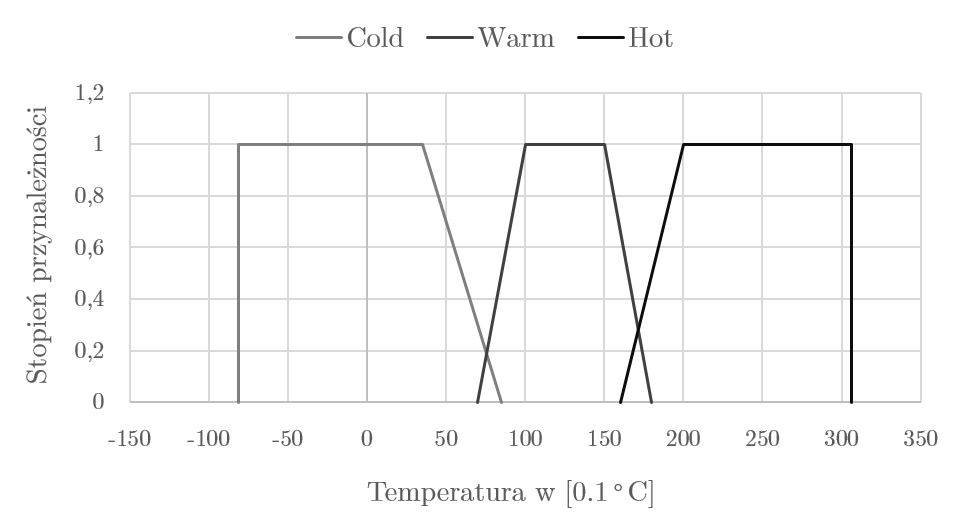
\includegraphics[width=0.99\textwidth]{Pictures/TermsCharts/TG_WJ.png}
	\caption{Wykres opisujący zmienną lingwistyczną dla kolumny TG dla pomiarów wykonanych astronomiczną wiosną i jesienią.}
\end{figure}

\begin{table}[H]
	\centering
	\begin{tabular}{c c c c c} 
		\hline
		\textbf{Etykieta} & \textbf{a} & \textbf{b} & \textbf{c} & \textbf{d}\\ [0.5ex] 
		\hline
		\hline 
Cold	 &-81 & -81 & 35 & 85 \\
Warm & 70 & 100 & 150 & 180 \\
Hot	 & 160 & 200 & 306 & 306 \\
		\hline
	\end{tabular}
	\caption{Przyporządkowane parametry funkcji trapezoidalnej dla zmiennej TGSA.}
\end{table}


Ostatnią zmienną dla kolumny TG będzie zmienna dotycząca pomiarów letnich - TGS.
\begin{figure}[H]
	\centering
	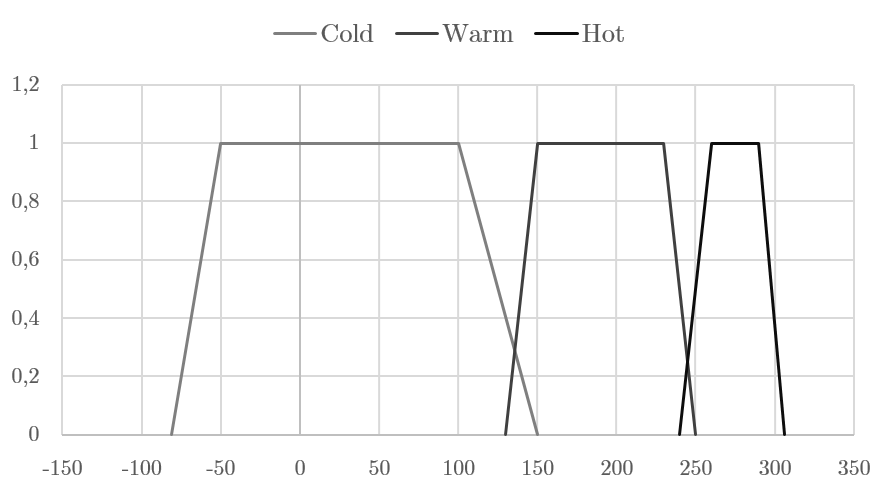
\includegraphics[width=0.99\textwidth]{Pictures/TermsCharts/TG_L.png}
	\caption{Wykres opisujący zmienną lingwistyczną dla kolumny TG dla pomiarów wykonanych astronomicznym latem.}
\end{figure}

\begin{table}[H]
	\centering
	\begin{tabular}{c c c c c} 
		\hline
		\textbf{Etykieta} & \textbf{a} & \textbf{b} & \textbf{c} & \textbf{d}\\ [0.5ex] 
		\hline
		\hline 
Cold	 &-81 & -81 & 100 & 150 \\
Warm & 130 & 150 & 230 & 250 \\
Hot	 & 240 & 260 & 306 & 306 \\
		\hline
	\end{tabular}
	\caption{Przyporządkowane parametry funkcji trapezoidalnej dla zmiennej TGS.}
\end{table}


\clearpage


\subsubsection{Kolumna TN}
Kolumna TN zawiera najniższą temperaturę powietrza w ciągu dnia. Wszystkie trzy warianty zmiennej lingwistycznej dla kolumny TN zaprezentowano poniżej:

\begin{itemize}[label=$\bullet$\scshape\bfseries]
\item TNW - dla pomiarów uzyskanych podczas astronomicznej zimy,
\item TNSA - dla pomiarów uzyskanych podczas astronomicznej wiosny lub jesieni,
\item TNS - dla pomiarów uzyskanych podczas astronomicznego lata.\newline\newline\newline
\end{itemize}


Pomiary zimowe - zmienna TNW.
\begin{figure}[H]
	\centering
	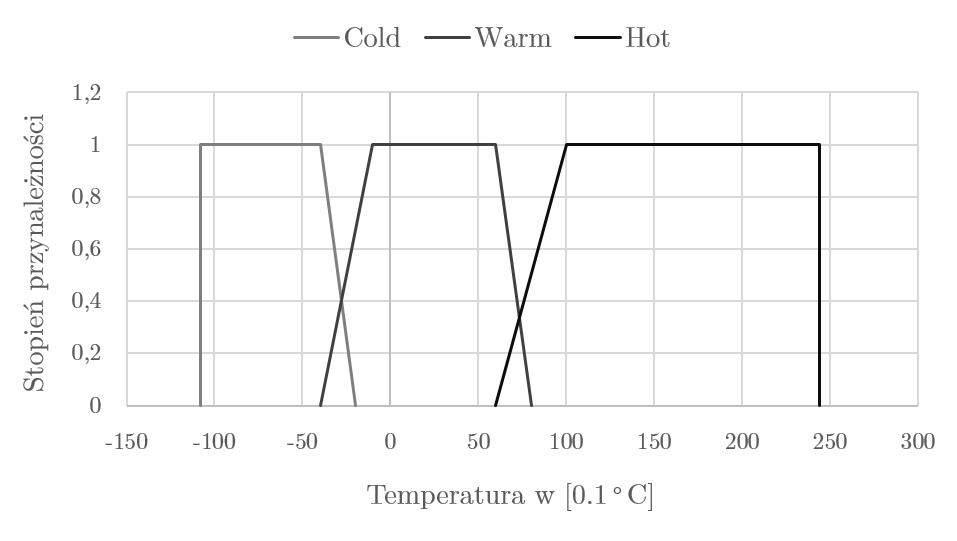
\includegraphics[width=0.99\textwidth]{Pictures/TermsCharts/TN_Z.png}
	\caption{Wykres opisujący zmienną lingwistyczną dla kolumny TN dla pomiarów wykonanych astronomiczną zimą.}
\end{figure}

\begin{table}[H]
	\centering
	\begin{tabular}{c c c c c} 
		\hline
		\textbf{Etykieta} & \textbf{a} & \textbf{b} & \textbf{c} & \textbf{d}\\ [0.5ex] 
		\hline
		\hline 
Cold	 &-108 & -108 & -40 & -20 \\
Warm & -40 & -10 & 60 & 80 \\
Hot	 & 60 & 100 & 244 & 244 \\
		\hline
	\end{tabular}
	\caption{Przyporządkowane parametry funkcji trapezoidalnej dla zmiennej TNW.}
\end{table}

Pomiary wiosenne i jesienne - zmienna TNSA.
\begin{figure}[H]
	\centering
	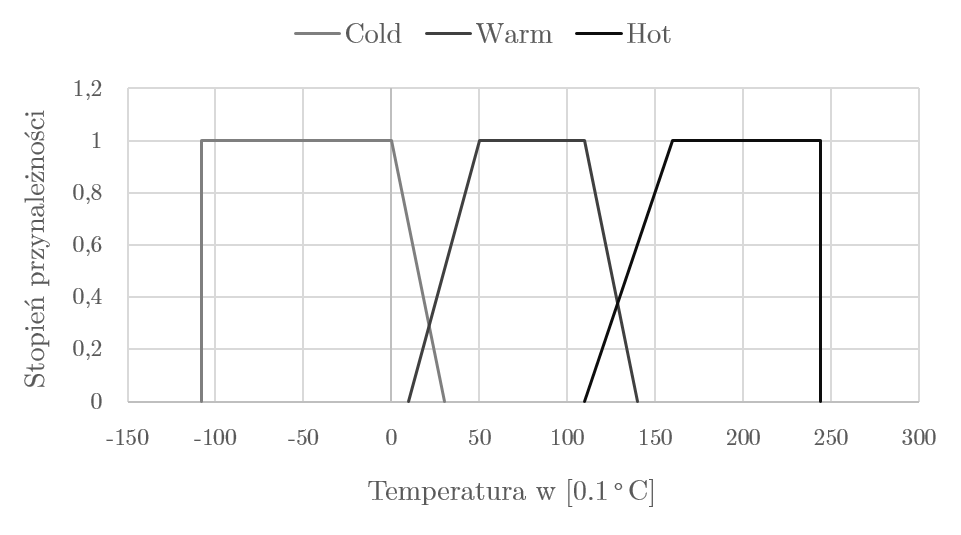
\includegraphics[width=0.99\textwidth]{Pictures/TermsCharts/TN_WJ.png}
	\caption{Wykres opisujący zmienną lingwistyczną dla kolumny TN dla pomiarów wykonanych astronomiczną wiosną i jesienią.}
\end{figure}

\begin{table}[H]
	\centering
	\begin{tabular}{c c c c c} 
		\hline
		\textbf{Etykieta} & \textbf{a} & \textbf{b} & \textbf{c} & \textbf{d}\\ [0.5ex] 
		\hline
		\hline 
Cold	 &-108 & -108 & 0 & 30 \\
Warm & 10 & 50 & 110 & 140 \\
Hot	 & 110 & 160 & 244 & 244 \\
		\hline
	\end{tabular}
	\caption{Przyporządkowane parametry funkcji trapezoidalnej dla zmiennej TNSA.}
\end{table}

Pomiary letnie - zmienna TNS.
\begin{figure}[H]
	\centering
	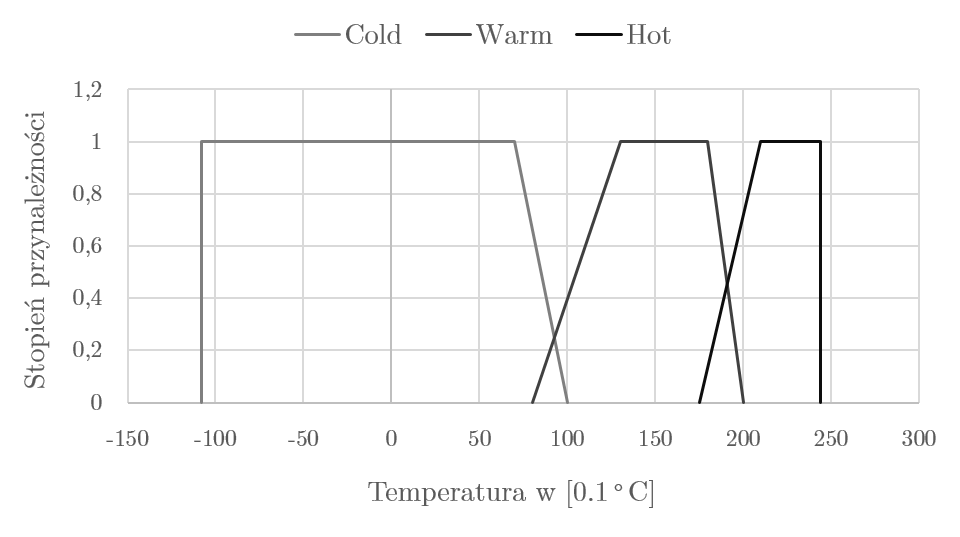
\includegraphics[width=0.99\textwidth]{Pictures/TermsCharts/TN_L.png}
	\caption{Wykres opisujący zmienną lingwistyczną dla kolumny TN dla pomiarów wykonanych astronomicznym latem.}
\end{figure}

\begin{table}[H]
	\centering
	\begin{tabular}{c c c c c} 
		\hline
		\textbf{Etykieta} & \textbf{a} & \textbf{b} & \textbf{c} & \textbf{d}\\ [0.5ex] 
		\hline
		\hline 
Cold	 &-108 & -108 & 70 & 100 \\
Warm & 80 & 130 & 180 & 200 \\
Hot	 & 175 & 210 & 244 & 244 \\
		\hline
	\end{tabular}
	\caption{Przyporządkowane parametry funkcji trapezoidalnej dla zmiennej TNS.}
\end{table}

\clearpage




\subsubsection{Kolumna TX}
Kolumna TX zawiera najwyższą temperaturę powietrza w ciągu dnia. Wszystkie trzy warianty zmiennej lingwistycznej dla kolumny TX zaprezentowano poniżej:

\begin{itemize}[label=$\bullet$\scshape\bfseries]
\item TXW - dla pomiarów uzyskanych podczas astronomicznej zimy,
\item TXSA - dla pomiarów uzyskanych podczas astronomicznej wiosny lub jesieni,
\item TXS - dla pomiarów uzyskanych podczas astronomicznego lata.\newline\newline\newline
\end{itemize}


Pomiary zimowe - zmienna TXW.
\begin{figure}[H]
	\centering
	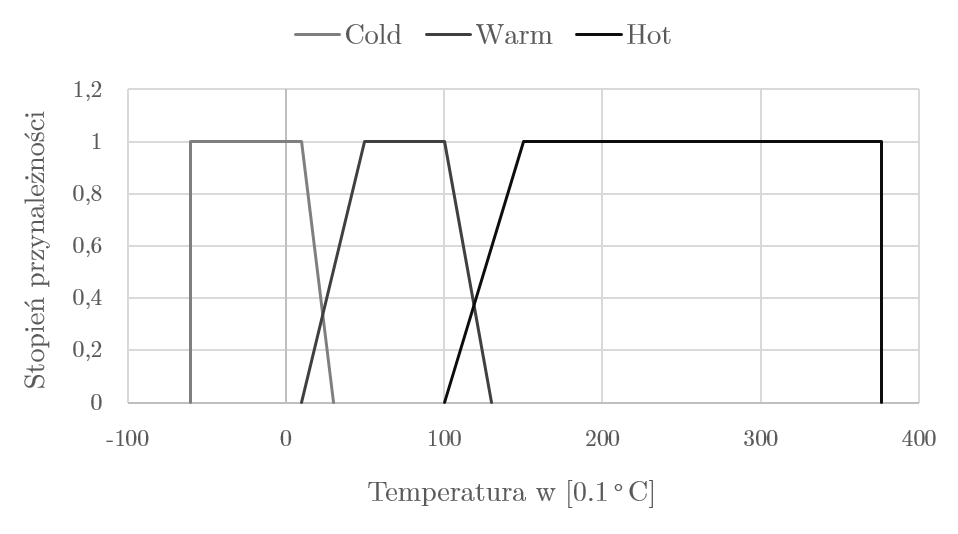
\includegraphics[width=0.99\textwidth]{Pictures/TermsCharts/TX_Z.png}
	\caption{Wykres opisujący zmienną lingwistyczną dla kolumny TX dla pomiarów wykonanych astronomiczną zimą.}
\end{figure}

\begin{table}[H]
	\centering
	\begin{tabular}{c c c c c} 
		\hline
		\textbf{Etykieta} & \textbf{a} & \textbf{b} & \textbf{c} & \textbf{d}\\ [0.5ex] 
		\hline
		\hline 
Cold	 &-60 & -60 & 10 & 30 \\
Warm & 10 & 50 & 100 & 130 \\
Hot	 & 100 & 150 & 376 & 376 \\
		\hline
	\end{tabular}
	\caption{Przyporządkowane parametry funkcji trapezoidalnej dla zmiennej TXW.}
\end{table}

Pomiary wiosenne i jesienne - zmienna TXSA.
\begin{figure}[H]
	\centering
	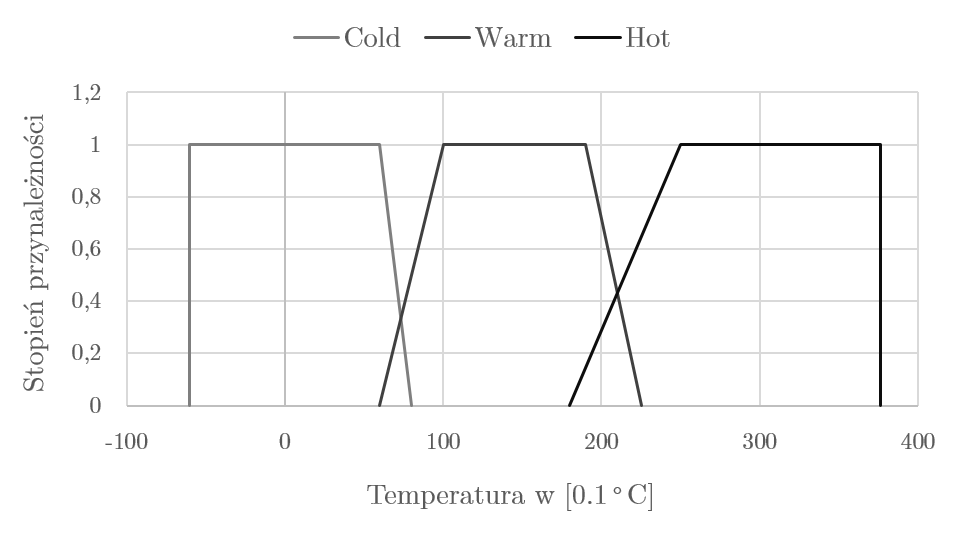
\includegraphics[width=0.99\textwidth]{Pictures/TermsCharts/TX_WJ.png}
	\caption{Wykres opisujący zmienną lingwistyczną dla kolumny TX dla pomiarów wykonanych astronomiczną wiosną i jesienią.}
\end{figure}

\begin{table}[H]
	\centering
	\begin{tabular}{c c c c c} 
		\hline
		\textbf{Etykieta} & \textbf{a} & \textbf{b} & \textbf{c} & \textbf{d}\\ [0.5ex] 
		\hline
		\hline 
Cold	 &-60 & -60 & 60 & 80 \\
Warm & 60 & 100 & 190 & 225 \\
Hot	 & 180 & 250 & 376 & 376 \\
		\hline
	\end{tabular}
	\caption{Przyporządkowane parametry funkcji trapezoidalnej dla zmiennej TXSA.}
\end{table}

Pomiary letnie - zmienna TXS.
\begin{figure}[H]
	\centering
	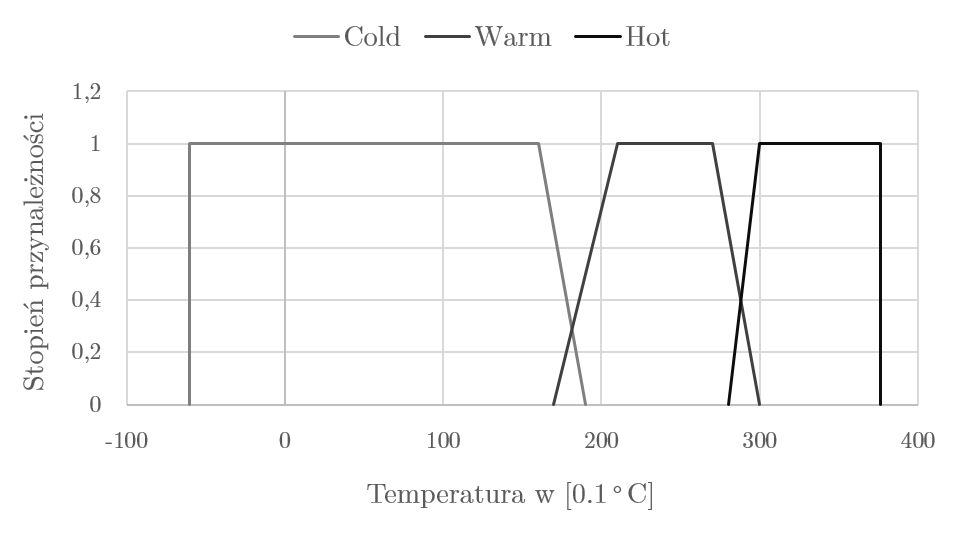
\includegraphics[width=0.99\textwidth]{Pictures/TermsCharts/TX_L.png}
	\caption{Wykres opisujący zmienną lingwistyczną dla kolumny TX dla pomiarów wykonanych astronomicznym latem.}
\end{figure}

\begin{table}[H]
	\centering
	\begin{tabular}{c c c c c} 
		\hline
		\textbf{Etykieta} & \textbf{a} & \textbf{b} & \textbf{c} & \textbf{d}\\ [0.5ex] 
		\hline
		\hline 
Cold	 &-60 & -60 & 160 & 190 \\
Warm & 170 & 210 & 270 & 300 \\
Hot	 & 280 & 300 & 376 & 376 \\
		\hline
	\end{tabular}
	\caption{Przyporządkowane parametry funkcji trapezoidalnej dla zmiennej TXS.}
\end{table}

\clearpage



\subsubsection{Kolumna T10N}
Kolumna T10N zawiera najmniejszą temperaturę w ciągu dnia zmierzoną na wysokości 10cm od poziomu gruntu. Wszystkie trzy warianty zmiennej lingwistycznej dla kolumny T10N zaprezentowano poniżej:

\begin{itemize}[label=$\bullet$\scshape\bfseries]
\item T10NW - dla pomiarów uzyskanych podczas astronomicznej zimy,
\item T10NSA - dla pomiarów uzyskanych podczas astronomicznej wiosny lub jesieni,
\item T10NS - dla pomiarów uzyskanych podczas astronomicznego lata.\newline\newline\newline
\end{itemize}


Pomiary zimowe - zmienna T10NW.
\begin{figure}[H]
	\centering
	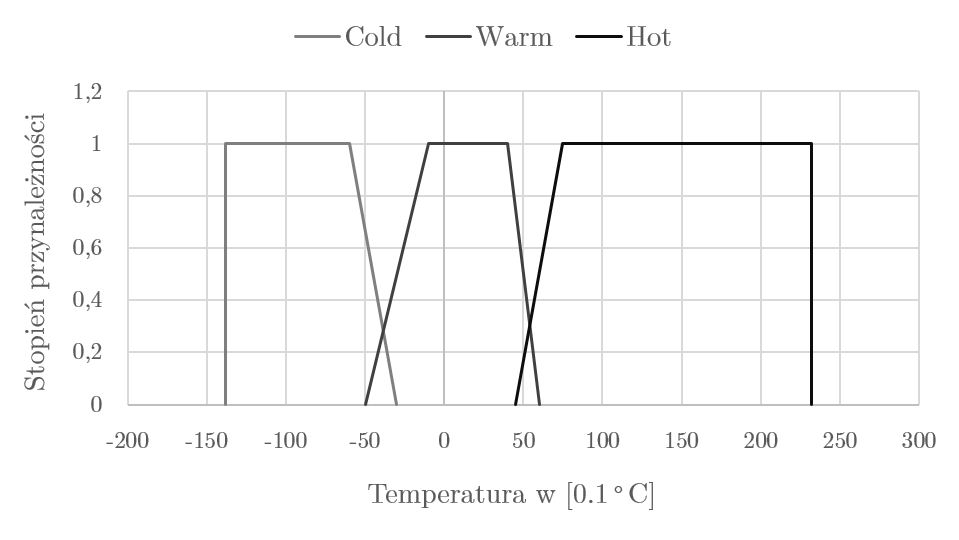
\includegraphics[width=0.99\textwidth]{Pictures/TermsCharts/T10_Z.png}
	\caption{Wykres opisujący zmienną lingwistyczną dla kolumny T10N dla pomiarów wykonanych astronomiczną zimą.}
\end{figure}

\begin{table}[H]
	\centering
	\begin{tabular}{c c c c c} 
		\hline
		\textbf{Etykieta} & \textbf{a} & \textbf{b} & \textbf{c} & \textbf{d}\\ [0.5ex] 
		\hline
		\hline 
Cold	 & -138 & -138 & -60 & -30 \\
Warm & -50 & -10 & 40 & 60 \\
Hot	 & 45 & 75 & 232 & 232 \\
		\hline
	\end{tabular}
	\caption{Przyporządkowane parametry funkcji trapezoidalnej dla zmiennej T10NW.}
\end{table}

Pomiary wiosenne i jesienne - zmienna T10NSA.
\begin{figure}[H]
	\centering
	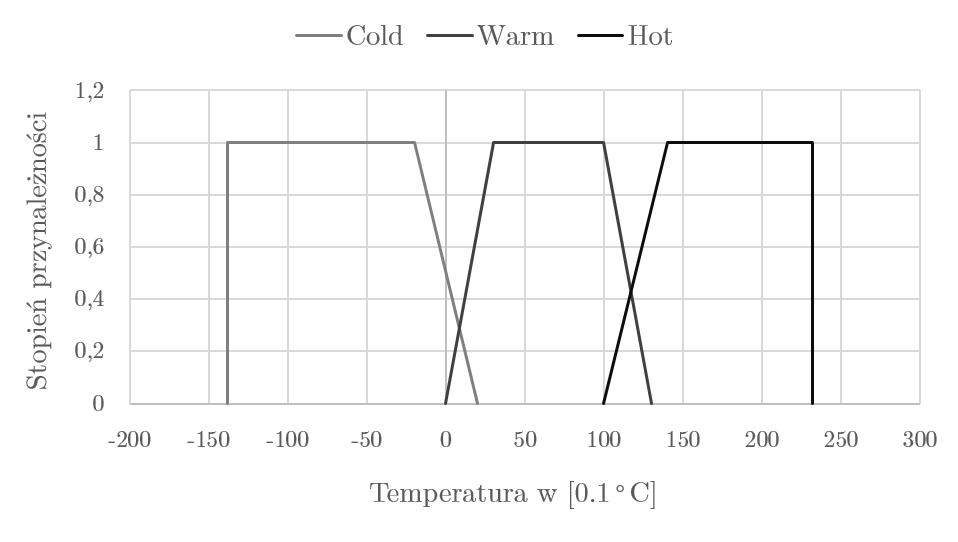
\includegraphics[width=0.99\textwidth]{Pictures/TermsCharts/T10_WJ.png}
	\caption{Wykres opisujący zmienną lingwistyczną dla kolumny T10N dla pomiarów wykonanych astronomiczną wiosną i jesienią.}
\end{figure}

\begin{table}[H]
	\centering
	\begin{tabular}{c c c c c} 
		\hline
		\textbf{Etykieta} & \textbf{a} & \textbf{b} & \textbf{c} & \textbf{d}\\ [0.5ex] 
		\hline
		\hline 
Cold	 & -138 & -138 & -20 & 20 \\
Warm & 0 & 30 & 100 & 130 \\
Hot	 & 100 & 140 & 232 & 232 \\
		\hline
	\end{tabular}
	\caption{Przyporządkowane parametry funkcji trapezoidalnej dla zmiennej T10NSA.}
\end{table}

Pomiary letnie - zmienna T10NS.
\begin{figure}[H]
	\centering
	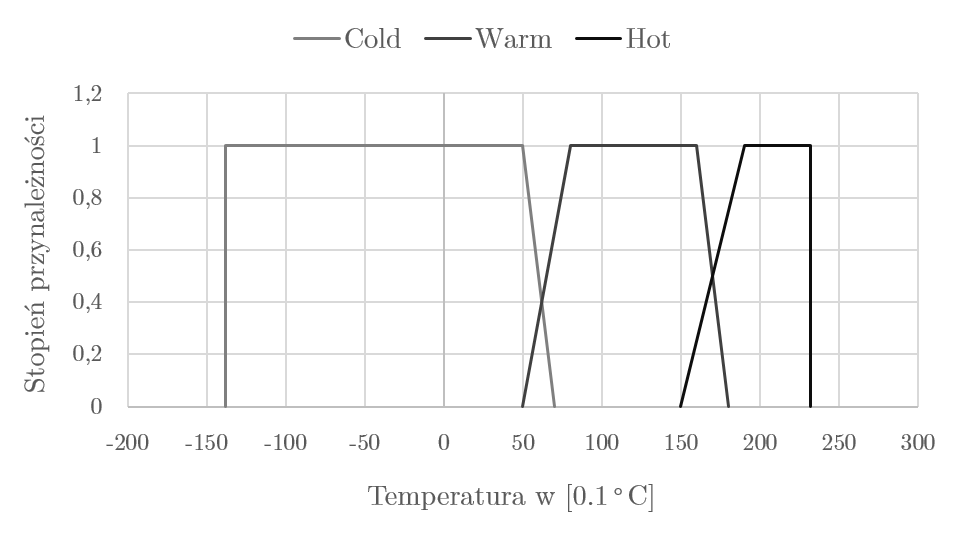
\includegraphics[width=0.99\textwidth]{Pictures/TermsCharts/T10_L.png}
	\caption{Wykres opisujący zmienną lingwistyczną dla kolumny T10N dla pomiarów wykonanych astronomicznym latem.}
\end{figure}

\begin{table}[H]
	\centering
	\begin{tabular}{c c c c c} 
		\hline
		\textbf{Etykieta} & \textbf{a} & \textbf{b} & \textbf{c} & \textbf{d}\\ [0.5ex] 
		\hline
		\hline 
Cold	 & -138 & -138 & 50 & 70 \\
Warm & 50 & 80 & 160 & 180 \\
Hot	 & 150 & 190 & 232 & 232 \\
		\hline
	\end{tabular}
	\caption{Przyporządkowane parametry funkcji trapezoidalnej dla zmiennej T10NS.}
\end{table}

\clearpage



\subsubsection{Kolumna Q}
Wykres opisujący zmienną lingwistyczną dla kolumny zawierającej wartości nasłonecznienia (Q), zamieszczono poniżej.
\begin{figure}[H]
	\centering
	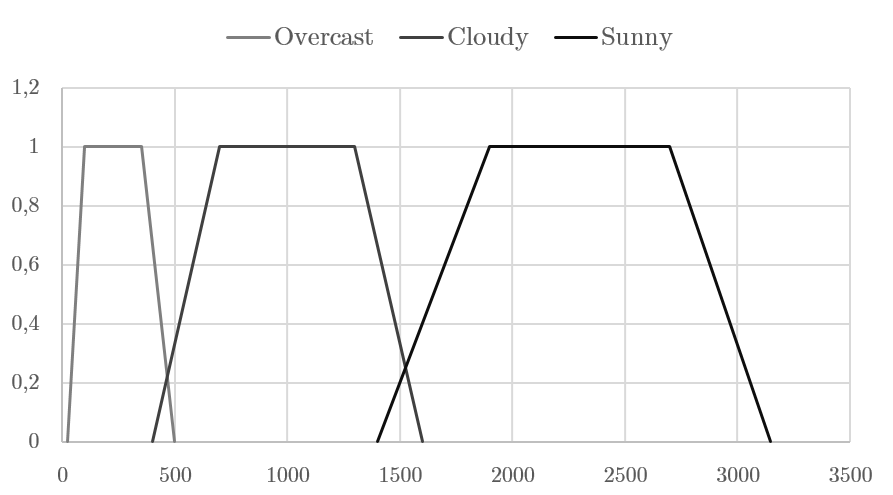
\includegraphics[width=0.99\textwidth]{Pictures/TermsCharts/Q.png}
	\caption{Wykres opisujący zmienną lingwistyczną dla kolumny Q}
\end{figure}

\begin{table}[H]
	\centering
	\begin{tabular}{c c c c c} 
		\hline
		\textbf{Etykieta} & \textbf{a} & \textbf{b} & \textbf{c} & \textbf{d}\\ [0.5ex] 
		\hline
		\hline 
Overcast	 & 24 & 24 & 350 & 500 \\
Cloudy & 400 & 700 & 1300 & 1600 \\
Sunny	 & 1400 & 1900 & 3145 & 3145 \\
		\hline
	\end{tabular}
	\caption{Przyporządkowane parametry funkcji trapezoidalnej dla kolumny Q.}
\end{table}

\clearpage



\subsubsection{Kolumna RH}
Wykres opisujący zmienną lingwistyczną dla kolumny zawierającej sumę opadów atmosferycznych w ciągu całego dnia (RH), zamieszczono poniżej.
\begin{figure}[H]
	\centering
	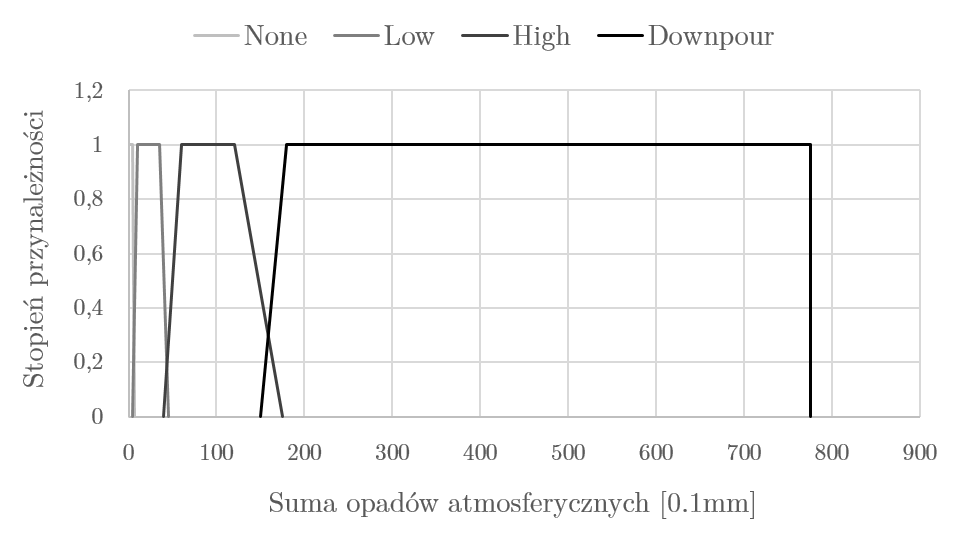
\includegraphics[width=0.99\textwidth]{Pictures/TermsCharts/RH.png}
	\caption{Wykres opisujący zmienną lingwistyczną dla kolumny RH}
\end{figure}

\begin{table}[H]
	\centering
	\begin{tabular}{c c c c c} 
		\hline
		\textbf{Etykieta} & \textbf{a} & \textbf{b} & \textbf{c} & \textbf{d}\\ [0.5ex] 
		\hline
		\hline 
None	 & -1 & -1 & 5 & 7 \\
Low 	& 5 & 10 & 35 & 45 \\
High		 & 40 & 60 & 120 & 175 \\
Downpour	 & 150 & 180 & 776 & 776 \\
		\hline
	\end{tabular}
	\caption{Przyporządkowane parametry funkcji trapezoidalnej dla kolumny RH.}
\end{table}

\clearpage




\subsection{Kwantyfikatory}
W tym rozdziale skoncentrujemy się na zaproponowanych przez nas kwantyfikatorach. Prezentację rozpoczniemy od kwantyfikatorów względnych, aby następnie omówić kwantyfikatory bezwzględne.\newline

W przypadku kwantyfikatorów, wykorzystywanymi przez nas funkcjami przynależności są zarówno funkcje trapezoidalne jak i funkcje trójkątne. Za każdym razem w tabelach podano, z jakiej funkcji skorzystano przy definicji danej etykiety, co ma swoje odzwierciedlenie na prezentowanych wykresach.

\subsubsection{Kwantyfikatory względne}
Wykres ilustrujący wszystkie kwantyfikatory względne, zamieszczono poniżej.
\begin{figure}[H]
	\centering
	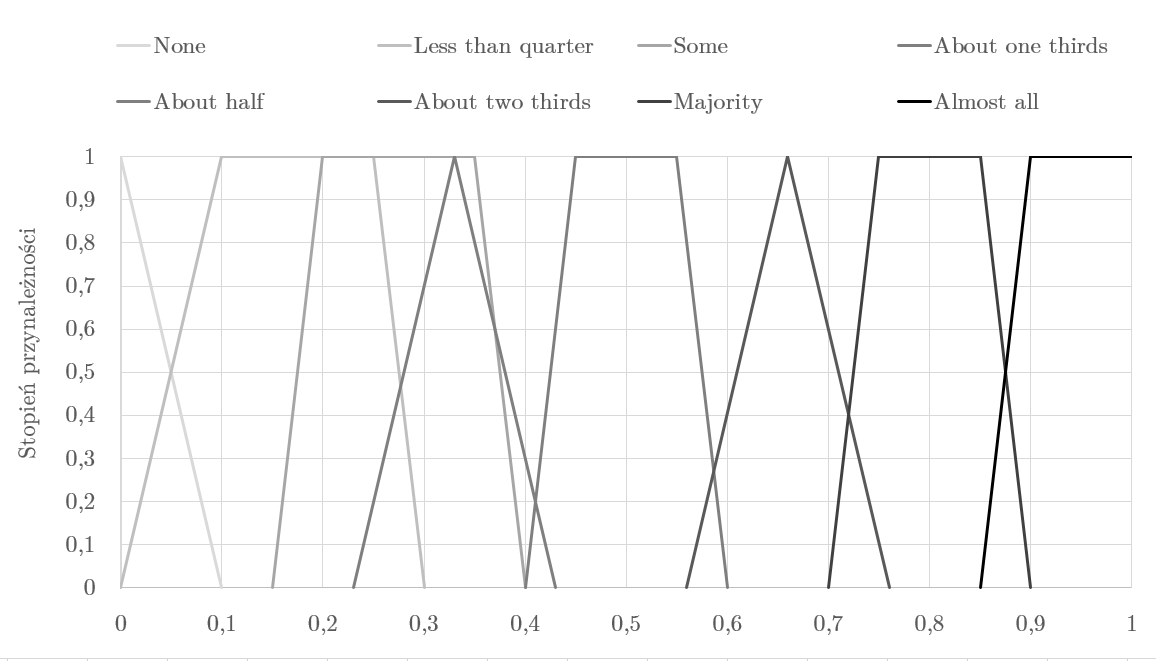
\includegraphics[width=0.99\textwidth]{Pictures/TermsCharts/nonabsolute.png}
	\caption{Kwantyfikatory względne}
\end{figure}

Tabela zawierająca parametry i nazwy funkcji przynależności, dla poszczególnych kwantyfikatorów, prezentuje się następująco.
\begin{table}[H]
	\centering
	\begin{tabular}{c c c c c c} 
		\hline
		\textbf{Kwantyfikator} & \textbf{Funkcja przynależności} & \textbf{a} & \textbf{b} & \textbf{c} & \textbf{d}\\ [0.5ex] 
		\hline
		\hline 
None	 			 & Trójkątna 		& 0 & 0 & 0.1 & - \\
Less than quarter		 & Trapezoidalna  	& 0 & 0.1 & 0.25 & 0.3 \\
Some				 & Trapezoidalna   & 0.15 & 0.2 & 0.35 & 0.4 \\
Around one thirds		 & Trójkątna 		& 0.23 & 0.33 & 0.43 & - \\
Around half	 		 & Trapezoidalna 	& 0.4 & 0.45 & 0.55 & 0.6 \\
Around two thirds		 & Trójkątna 		& 0.56 & 0.66 & 0.67 & - \\
Majority	 			 & Trapezoidalna 	& 0.7 & 0.75 & 0.85 & 0.9 \\
Almost all			 & Trapezoidalna 	& 0.85 & 0.9 & 1 & 1 \\
		\hline
	\end{tabular}
	\caption{Funkcje przynależności kwantyfikatorów względnych - nazwy wraz z parametrami.}
\end{table}


\subsubsection{Kwantyfikatory bezwzględne}
Wykres ilustrujący wszystkie kwantyfikatory bezwzględne, zamieszczono poniżej.
\begin{figure}[H]
	\centering
	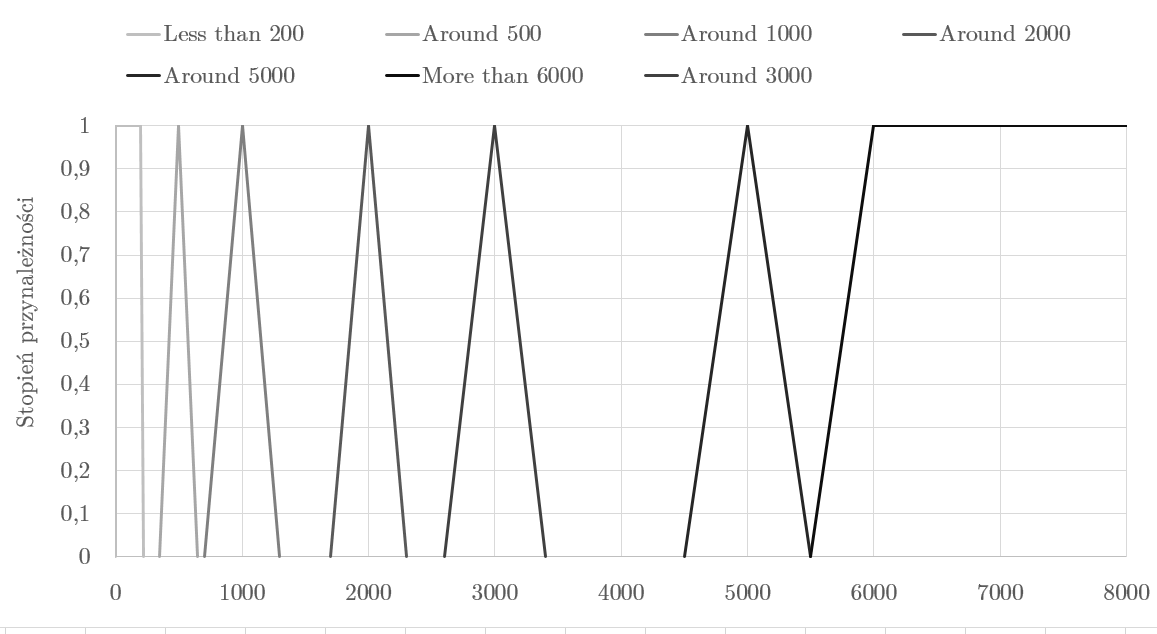
\includegraphics[width=0.99\textwidth]{Pictures/TermsCharts/absolute.png}
	\caption{Kwantyfikatory bezwzględne}
\end{figure}

Tabela zawierająca parametry i nazwy funkcji przynależności, dla poszczególnych kwantyfikatorów, prezentuje się następująco.
\begin{table}[H]
	\centering
	\begin{tabular}{c c c c c c} 
		\hline
		\textbf{Kwantyfikator} & \textbf{Funkcja przynależności} & \textbf{a} & \textbf{b} & \textbf{c} & \textbf{d}\\ [0.5ex] 
		\hline
		\hline 
Less than 200	 	& Trapezoidalna 		& 0 & 0 & 200 & 220 \\
Around 500			& Trójkątna  			& 350 & 500 & 650 & - \\
Around 1000		      & Trójkątna   			& 700 & 1000 & 1300 & - \\
Around 2000	 		& Trójkątna 			& 1700 & 2000 & 2300 & - \\
Around 3000 		 	& Trójkątna 			& 2600 & 3000 & 3400 & - \\
Around 5000	 		& Trójkątna 			& 4500 & 5000 & 5500 & - \\
More than 6000		& Trapezoidalna 		& 5500 & 6000 & 8000 & 17000 \\
		\hline
	\end{tabular}
	\caption{Funkcje przynależności kwantyfikatorów bezwzględnych - nazwy wraz z parametrami.}
\end{table}

\clearpage





\section{Wyniki}

Przeprowadzone eksperymenty zostały podzielone na trzy etapy, w których porównywać będziemy różne zależności:
\begin{itemize}[label=$\bullet$\scshape\bfseries]
\item W pierwszym etapie sprawdzimy jak zmieniać się będą miary podsumowań dla poszczególnych kwantyfikatorów.
\item W drugim etapie przeanalizujemy zdania bardziej złożone - sumaryzatory wykorzystujące spójniki \emph{AND} oraz \emph{OR}.
\item W trzecim etapie skoncentrujemy się na różnicy w rezultatch uzyskiwanych w wyniku wykorzystania kwalifikatora w opozycji do zdań, w których kwalifikator nie jest używany.
\end{itemize}


\subsection{Wpływ wyboru kwantyfikatora na jakość podsumowania}

W pierwszym etapie, wygenerowano następujące zdania:
\begin{itemize}[label=$\bullet$\scshape\bfseries]
\item Zdanie pierwsze: \textit{X of summer measures with cold daily average temperature have cloudy insolation} - wykorzystujące zmienną lingwistyczną TGS jako kwalifikator (etykieta \textit{Cold}) oraz zmienną Q jako sumaryzator (etykieta \textit{Cloudy}).
\item Zdanie drugie: \textit{X of measures with very strong strongest wind blow have overcast insolation} - wykorzystujące zmienną lingwistyczną FXX jako kwalifikator (etykieta \textit{Very strong}) oraz zmienną Q jako sumaryzator (etykieta \textit{Overcast}).
\item Zdanie trzecie: \textit{X of measures with none precipitation have gentle daily wind speed average.} - wykorzystujące zmienną lingwistyczną RH jako kwalifikator (etykieta \textit{None}) oraz zmienną FG jako sumaryzator (etykieta \textit{Gentle}).
\end{itemize}
gdzie \textit{X} jest jednym ze zdefiniowaych przez nas kwantyfikatorów.\newline

Miary $T_2 - T_5$ oraz $T_8 - T_{11}$ osiągały stałe wartości w obrębie każdego ze zdań, dlatego też ich wartości zostały zamieszczone poza tabelami, w których zestawiono tylko te miary, których wartości były zmienne wewnątrz jednego eksperymentu.

\subsubsection{Zdanie pierwsze}

\begin{table}[H]
	\centering
	\begin{tabular}{c c c c} 
		\hline
		\textbf{Kwantyfikator}  & \textbf{$T_1$} & \textbf{$T_6$} & \textbf{$T_7$}\\ [0.5ex] 
		\hline
None	&	0,000	&	0,900	&	0,950	\\
Less than quarter	&	0,000	&	0,700	&	0,775	\\
Some 	&	0,000	&	0,750	&	0,800	\\
Around one thirds 	&	0,000	&	0,800	&	0,900	\\
Around half 	&	0,000	&	0,800	&	0,850	\\
Around two thirds 	&	0,116	&	0,800	&	0,900	\\
Majority 	&	0,968	&	0,800	&	0,850	\\
Almost all	&	0,000	&	0,840	&	0,870	\\
Less than 200	&	1,000	&	0,950	&	0,953	\\
Around 500	&	0,000	&	0,932	&	0,966	\\
Around 1000	&	0,000	&	0,865	&	0,932	\\
Around 2000	&	0,000	&	0,865	&	0,932	\\
Around 3000	&	0,000	&	0,820	&	0,910	\\
Around 5000	&	0,000	&	0,775	&	0,887	\\
More than 6000	&	0,000	&	-1,590	&	-0,520	\\
		\hline
	\end{tabular}
	\caption{Tabela przedstawiająca wyniki eksperymentu dla zdania pierwszego}
\end{table}

\subsubsection{Zdanie drugie}

\subsubsection{Zdanie trzecie}



\subsection{Wpływ wykorzystania operacji sumy i ilooczynu na jakość podsumowania}
\textit{Praca w toku}

\subsection{Wpływ wykorzystania kwalifikatora na jakość podsumowania}
\textit{Praca w toku}




\section{Dyskusja}
\textit{Praca w toku}


\section{Wnioski}
\textit{Praca w toku}


\begin{thebibliography}{2}
\bibitem{baza} 
Baza danych - 
\href{https://www.kaggle.com/sinaasappel/historical-weather-in-the-netherlands-19012018}{\textit{"Historical weather in the Netherlands 1901-2018"}}
\bibitem{Maven} 
Narzędzie Maven\newline
\textit{https://maven.apache.org/}. 
\bibitem{FX} 
Biblioteka JavaFX\newline
\textit{https://openjfx.io/}
\bibitem{ksiazka}
Methods for the linguistic summarization of data - aplications of fuzzy sets and their extensions, Adam Niewiadomski, Akademicka Oficyna Wydawnicza EXIT, Warszawa 2008
\end{thebibliography}
\end{document}
